
\newcommand{\ConstExercise}{5}
\newcommand{\ConstDeadline}{12.05.2023}

\documentclass[11pt,letterpaper]{article}
\textwidth 6.5in
\textheight 9.in
\oddsidemargin 0in
\headheight 0in

\usepackage[exp]{custom_0.1}

\begin{document}

%%%%% Document %%%%%

\begin{enumerate}
    \item \textbf{Ideales und reales Gas}\,\\[1ex]
        Als ideales Gas:
        \begin{align*}
            p_{i}= \frac{N k_B T}{V}
            = \frac{n R T}{V}
        \end{align*}
        
        Als reales Gas:
        \begin{align*}
            n R T &= \left(p+\frac{a n^2}{V^2}\right) \cdot(V-n b)\\\
            p_r &= \frac{n R T}{V-n b} - \frac{a n^2}{V^2}
        \end{align*}

        Relativer Fehler:
        \begin{align*}
            \delta_{rel} &= \frac{p_i}{p_r} - 1
            = \frac{\frac{n R T}{V}}{\frac{n R T}{V-n b} - \frac{a n^2}{V^2}} - 1
            = \frac{R T}{\frac{R V T}{V-n b} - \frac{a n}{V}} - 1\\
            \delta_{rel}(V=2\,\mathrm{l})&\approx \frac{\cug \cdot 293.15\,\mathrm{K}}{\frac{\cug \cdot 2\cdot0.1^3\,\mathrm{m^3} \cdot 293.15\,\mathrm{K}}{2\cdot0.1^3\,\mathrm{m^3}-1\,\mathrm{mol}\cdot 3.22\cdot 10^{-1}\ufrac{m^3}{mol}} - \frac{1\,\mathrm{mol}\cdot 0.136\,\ufrac{Pa\,m^6}{mol^2}}{2\cdot0.1^3\,\mathrm{m^3}}} - 1\\
            &\approx 1.17\%\\
            \delta_{rel}(V=0.2\,\mathrm{l})&\approx \frac{\cug \cdot 293.15\,\mathrm{K}}{\frac{\cug \cdot 0.2\cdot0.1^3\,\mathrm{m^3} \cdot 293.15\,\mathrm{K}}{0.2\cdot0.1^3\,\mathrm{m^3}-1\,\mathrm{mol}\cdot 3.22\cdot 10^{-1}\ufrac{m^3}{mol}} - \frac{1\,\mathrm{mol}\cdot 0.136\,\ufrac{Pa\,m^6}{mol^2}}{0.2\cdot0.1^3\,\mathrm{m^3}}} - 1\\
            &\approx 9.54\%
        \end{align*}
    
    \item \textbf{Schlittschuhläuferin}
        \begin{align*}
            Q &= T\cdot \derivative{p_S}{T} \cdot (V_G - V_L)\\
            \int_{T_0}^{T_1} \frac{Q}{T} \,\di T&= \int_{T_0}^{T_1} \derivative{p_S}{T} \cdot (V_G - V_L)\\
            \int_{T_0}^{T_1} \frac{Q}{T} \,\di T &= \int_{p_0}^{p_1}(V_G - V_L)\, \di p_S\\
             Q \ln\cbrace{\frac{T_1}{T_0}} &= (V_G - V_L)(p_1 - p_0)
        \end{align*}
        \newpage
        \begin{align*}
            T_{1} &= T_{0} \cdot e^{\frac{\Delta p (V_W - V_E)}{q_W}}\\
            &= T_{0} \cdot e^{\frac{m g (V_W - V_E)}{A q_W}}\\
            &\approx 273.15 \,\mathrm{K} \cdot e^{\frac{65\mathrm{kg} \cdot 9.81 \ufrac{m}{s^2} \cbrace{10^{-3}\,\ufrac{m^3}{kg} - 1.091\cdot10^{-3}\,\ufrac{m^3}{kg}}}{2\cdot 10^{-5} \,\mathrm{m^2}\cdot 334\cdot 10^{3} \ufrac{J}{kg}}}\\
            &\approx 271 \,\mathrm{K}\\
        \end{align*}

    
    \item \textbf{Van-der-Waals-Gleichung}
        \begin{enumerate}
            \item
            \begin{align*}
                p &= \frac{N k T}{V - N b} - \frac{a N^2}{V^2}\\
                \\
                \partiald{p}{V} &= 0 = -\frac{N k T}{(V - N b)^2} +  \frac{2 a N^2}{V^3}\\
                &= -N k T V^3 +  2 a N^2(V - N b)^2\\
                T &=  \frac{2 a N^2(V - N b)^2}{k N V^3}=  \frac{2 a N(V - N b)^2}{k V^3}\\\\
                \\
                \partiald{^2p}{V^2} &= 0 =  \frac{2 N k T}{(V - N b)^3} -  \frac{6 a N^2}{V^4}\\
                &=  2 N k T V^4 -  6 a N^2 (V - N b)^3\\
                &=  2 N k \frac{2 a N(V - N b)^2}{k V^3} V^4 -  6 a N^2 (V - N b)^3\\
                &= 2 V -  3 (V - N b)\\
                V_C &= 3 N b\\
                \\
                T_C &=  \frac{2 a N(3 N b - N b)^2}{k (3 N b)^3}\\
                &=  \frac{8 a N^3 b^2}{27 k N^2 b^3}\\
                &=  \frac{8 a}{27 k b}\\
                N k T_C &=  \frac{8 a N}{27 b}\\
            \end{align*}
            \begin{align*}
                p_C &= \frac{\frac{8 a N}{27 b}}{3 N b - N b} - \frac{a N^2}{(3 N b)^2}\\
                &= \frac{4 a}{27 b^2} - \frac{a}{9 b^2}\\
                &= \frac{a}{27 b^2} \\
            \end{align*}

            \item
            \begin{align*}
                \begin{cases}
                    x = \frac{V}{V_C}\\
                    y = \frac{p}{p_C}\\
                    z = \frac{T}{T_C}\\
                \end{cases} &\Longrightarrow
                \begin{cases}
                    x V_C = V\\
                    y p_C = p\\
                    z T_C = T\\
                \end{cases}\\
                p &= \frac{N k T}{V - N b} - \frac{a N^2}{V^2}\\
                y p_C &= \frac{N k z T_C}{x V_C - N b} - \frac{a N^2}{x^2 V_C^2}\\
                y &= \frac{N k z T_C}{ p_C (x V_C - N b)} - \frac{a N^2}{x^2 V_C^2 p_C}\\
                y &= \frac{z \frac{8 a N}{27 b}}{ \frac{a}{27 b^2} (x \cdot3 N b - N b)} - \frac{a N^2}{x^2 (3 N b)^2 \frac{a}{27 b^2}}\\
                y &= \frac{8 z}{3x - 1} - \frac{3}{x^2}\\
            \end{align*}
            Der Vorteil dieser Gleichung liegt darin, dass materialabhängige und skalenabhängige Effekte rausgerechnet werden, 
            d.h. es wurde eine Gleichung gefunden, die in identischer Form für alle Stoffe gilt,
            die die Van-der-Waals-Gleichung befolgen.
        \end{enumerate}
    
    
    \item \textbf{Ladung im Quadrat}
        \begin{enumerate}
            \item 
            Der Versuch sei wie folgt angeordnet:
            \begin{align*}
                \begin{array}{ccc}
                    q_1 & q_3 &\\
                    q_2 & q_4 &\\
                    &&p
                \end{array}
            \end{align*}
            Wobei $q_i$ die Ladungen sind, und $p$ der Ort ist für den die Feldstärke
            ausgerechnet werden soll. 

            Aufgrund der Symmetrie entlang der Linie von $q_1$ nach $q_4$, 
            kann es nur eine Kraftkomponente in Richtung des Mittelpunktes 
            der vier Ladungen geben. Diese Richtung soll mit $\e_m$ angegeben werden.

            \begin{align*}
                \vec{E}(p) &= \e_m\cbrace{E_{q_1}(p) + E_{q_2}(p) + E_{q_3}(p) + E_{q_4}(p)}\\
                \vec{E_{q_1}}(p) &= \e_m k \frac{Q}{r_{q_1,p}^2} = k \frac{Q}{\cbrace{2a + \frac{a}{\sqrt{2}}}^2}\\
                \vec{E_{q_4}}(p) &= \e_m k \frac{Q}{r_{q_4,p}^2} = k \frac{Q}{\cbrace{2a - \frac{a}{\sqrt{2}}}^2}\\
                \vec{E_{q_2}}(p) \cdot \e_m &= E_{q_3}(p) \cdot \e_m  
                = \cos(\alpha) k \frac{Q}{r_{q_3,p}^2} \\
                &= \e_m \cos\cbrace{\arctan^{-1}\cbrace{\frac{\frac{a}{\sqrt{2}}}{2a}}} k \frac{Q}{(2a)^2 + (\frac{a}{2\sqrt{2}})^2}\\
                &= \e_m \cos\cbrace{\arctan^{-1}\cbrace{\frac{1}{2\sqrt{2}}}} k \frac{Q}{(2a)^2 + (\frac{a}{2\sqrt{2}})^2}\\
            \end{align*} 
            \begin{align*}
                \vec{E}(p) &= \e_m k \frac{Q}{\cbrace{2a + \frac{a}{\sqrt{2}}}^2}
                +  \e_m k \frac{Q}{\cbrace{2a - \frac{a}{\sqrt{2}}}^2}
                + 2\e_m \cos\cbrace{\arctan^{-1}\cbrace{\frac{1}{2\sqrt{2}}}} k \frac{Q}{(2a)^2 + (\frac{a}{2\sqrt{2}})^2}\\
                &= k Q \e_m \cbrace{\frac{1}{\cbrace{2a + \frac{a}{\sqrt{2}}}^2}
                +  \frac{1}{\cbrace{2a - \frac{a}{\sqrt{2}}}^2}
                + 2 \cos\cbrace{\arctan^{-1}\cbrace{\frac{1}{2\sqrt{2}}}} \frac{1}{(2a)^2 + (\frac{a}{2\sqrt{2}})^2}}\\
                &\approx \e_m 8.99\cdot 10^{9}\, \ufrac{Nm^2}{C^2} \cdot 40\cdot 10^{-6} \, \mathrm{C} \left(\frac{1}{\cbrace{4\,\mathrm{m} + \frac{2\,\mathrm{m}}{\sqrt{2}}}^2}
                +  \frac{1}{\cbrace{4\,\mathrm{m} - \frac{2\,\mathrm{m}}{\sqrt{2}}}^2}+\right.\\
                &\qquad \qquad\qquad\qquad\qquad\qquad\qquad\qquad \left.2\cdot \cos\cbrace{\arctan^{-1}\cbrace{\frac{1}{2\sqrt{2}}}} \frac{1}{(4\,\mathrm{m})^2 + (\frac{2\,\mathrm{m}}{2\sqrt{2}})^2}\right)\\
                &\approx \e_m 1.07\cdot 10^{5}\,\ufrac{N}{C}\\
            \end{align*}

            \item
            Aufgrund der Symmetrie des Problems gleichen sich die Beiträge jedes 
            geladenen Teilchens mit dem des gegenübergelegenden aus - Das E-Feld 
            kann also nur gleich null sein $(\vec{E}(m)=\vec{0})$.
        \end{enumerate}

    
    \item \textbf{Milikan-Versuch}
        \begin{enumerate}
            \item
            Der Milikan-Versuch ist ein 1907 von Robert C. Milikan durchgeführter
            Versuch zur Bestimmung der Elementarladung. Er funktioniert wie folgt:
            \begin{enumerate}
                \item Es werden kleine Öltröpfchen in eine Kammer gesprüht. Durch Reibung und
                 andere Effekte sind diese meist nicht ganz neutral geladen.
                \item Anschließend wird die Masse von einzelnen Tröpfchen bestimmt, indem die maximale
                Fallgeschwindigkeit über das Stoke'sche Reibungsgesetz mit der Masse in
                Verbindung gebracht wird.
                \item Nun kommt es zum letzten Schritt des eigentlichen Experimentes: Man stellt das elektrische Feld eines Kondensators
                so ein, dass es die Schwerkraft für ein gegebenes Teilchen perfekt kompensiert und notiert diese E-Feld-Stärke. 
                \item Schließlich muss noch ein wenig ausgewertet werden. Mit den gesammelten Messdaten als Grundlage
                lassen sich nun die Ladungen verschiedener Öltröpchen ausrechenen und plotten. Es wird auffallen, 
                das diese nur in ganzzahligen Vielfachen einer konstanten Zahl, der sogenannten Elementarladung, auftritt.
            \end{enumerate}

            \item \,
            \begin{figure*}[h!]
                \begin{center}
                    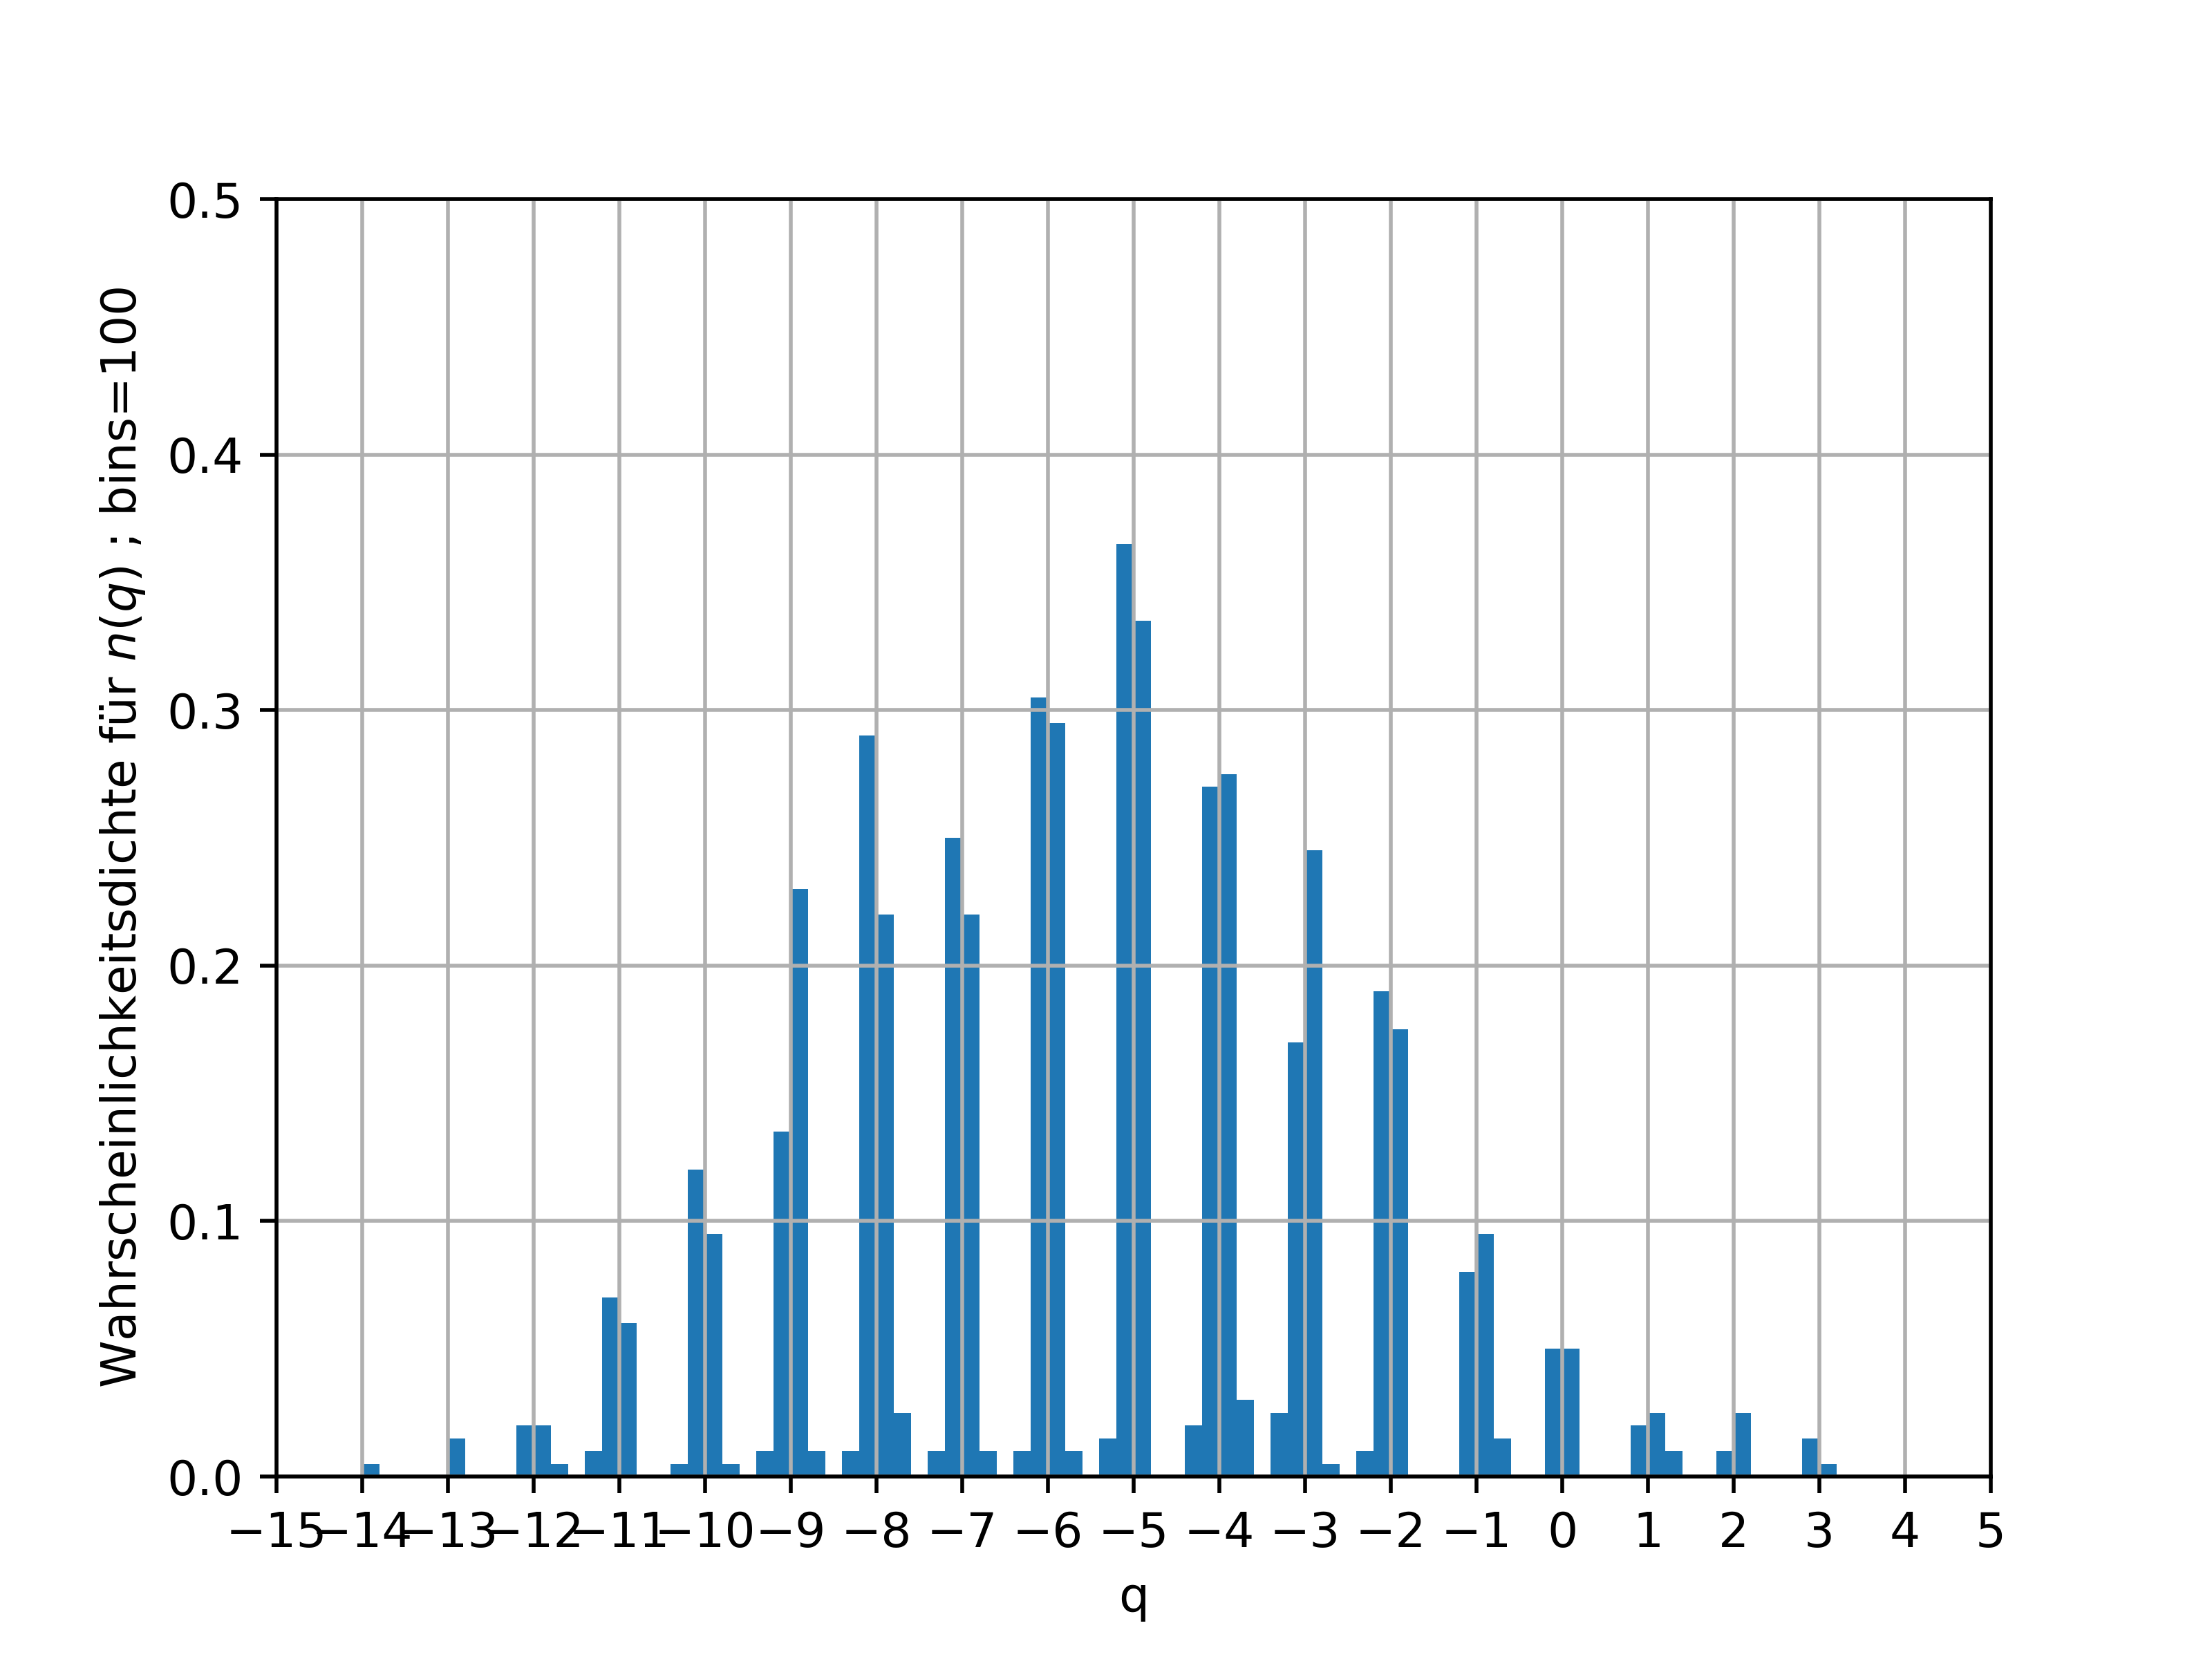
\includegraphics[width = 0.75\textwidth]{hist}
                \end{center}
            \end{figure*}

            \item
            \begin{align*}
                F &= F_S^R + F_A +F_G = 0\\
                F_S^R &= -\kappa v = - 6\pi \eta r v\\
                F_A &= -V \rho_{Luft} g\\
                F_G &= V \rho_{Ol} g\\
                \\
                F &= 0 = - 6\pi \eta r v
                - V \rho_{Luft} g
                + V \rho_{Ol} g\\ 
                &= - 6\pi \eta r v
                - \frac{4}{3}\pi r^3 \rho_{Luft} g
                + \frac{4}{3}\pi r^3 \rho_{Ol} g\\
                &= - \frac{9}{2} \eta  v
                +  r^2 g \cbrace{\rho_{Ol} - \rho_{Luft} } \\ 
                r &= \sqrt{\frac{9}{2} \frac{\eta  v}{ g \cbrace{\rho_{Ol} - \rho_{Luft} }} }\\ 
             \end{align*}

            \item
            \begin{align*}
                F_G &=  F_A + F_E\\
                V \rho_{Ol} g &= -V\rho_{Luft} g + q E\\
                q &= V g\frac{\rho_{Ol} - \rho_{Luft}}{E}\\
                &= \frac{4}{3}\pi r^3 \cdot g d \frac{\rho_{Ol} - \rho_{Luft}}{U}\\
                &= \frac{4}{3}\pi \cbrace{\frac{9}{2} \frac{\eta  v}{ g \cbrace{\rho_{Ol} - \rho_{Luft} }} }^{\frac{3}{2}} \cdot g d \frac{\rho_{Ol} - \rho_{Luft}}{U}\\
                &= \frac{9\pi d }{U} \sqrt{ \frac{2 \eta^3  v^3}{ g \cbrace{\rho_{Ol} - \rho_{Luft} }} }\\
            \end{align*}

            \item
            Man könnte die Spannung nur langsam hochdrehen, und aufhören sobald
            die ersten Tröpfchen anfangen zu schweben. So würde man nur die Tröpfchen
            mit der geringsten Ladungmenge betrachten, die, unter der 
            Annahme eines angemessenden Versuchumfangs, der Elementarladung
            entsprechen sollte. 

        \end{enumerate}
\end{enumerate}

\end{document}